\appendix
\chapter{Dados utilizados para calibração}
\label{sec:apendice}
Nesta secção serão apresentados os dados complementares utilizados para a calibração dos experimentos.

Para melhor organização os experimentos realizados serão divididos em: "Experimento I", "Experimento II", "Experimento III" e "Experimento IV".

\section{Experimento I}
A tabela e os dados utilizados para a calibração do espectro com LED desligado, já foram apresentadas na secção \ref{sec:result_producao_cluster}. A calibração do espectro com LED ligado pode ser vista na Figura \ref{fig:01_calib_ledON}.

\begin{figure}
  \centering  
  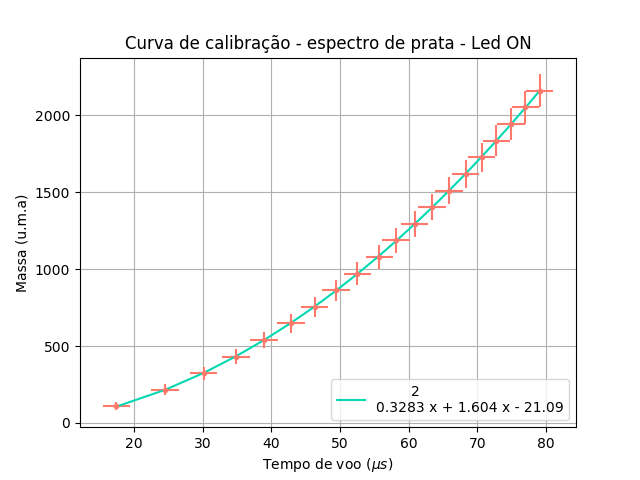
\includegraphics[width=0.7\textwidth]{exp_01/LEDON_curv+erro_calib.png}
  \caption{Curva de calibração para o LED ligado.}
  \label{fig:01_calib_ledON} 
\end{figure}

Utilizando o processamento de dados foi obtido o espectro de partículas em função do tempo e em função da massa, como pode ser visto respectivamente nas Figuras \ref{fig:01_ledon_dados_tratados} e \ref{fig:01_ledon_massa}.

\begin{figure}
  \centering  
  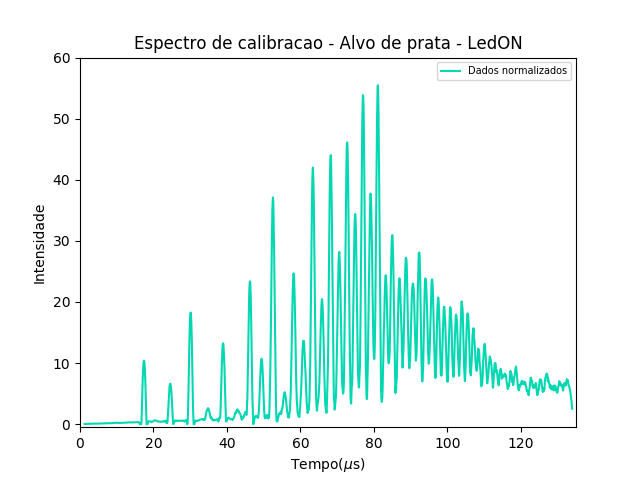
\includegraphics[width=0.7\textwidth]{exp_01/LedON_normalizado_mcp.png}
  \caption{Espectro de calibração com tratamento de dados.}
  \label{fig:01_ledon_dados_tratados} 
\end{figure}

\begin{figure}
  \centering  
  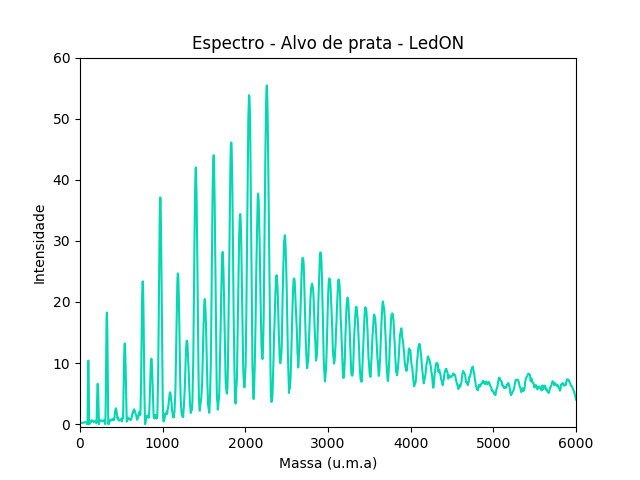
\includegraphics[width=0.7\textwidth]{exp_01/LEDON_espec_calib_ag_massa.png}
  \caption{Espectro de calibração com tratamento de dados.}
  \label{fig:01_ledon_massa} 
\end{figure}


\section{Experimento II}
A tabela e os dados utilizados para a calibração de ambos os estados do LED, pode ser vista na Tabela \ref{tab:picos_encontados_02}, assim como as curvas de calibração dos espectros que correspondem as Figuras \ref{fig:02_calib_ledOFF} e \ref{fig:02_calib_ledON}.

\begin{figure}
  \centering  
  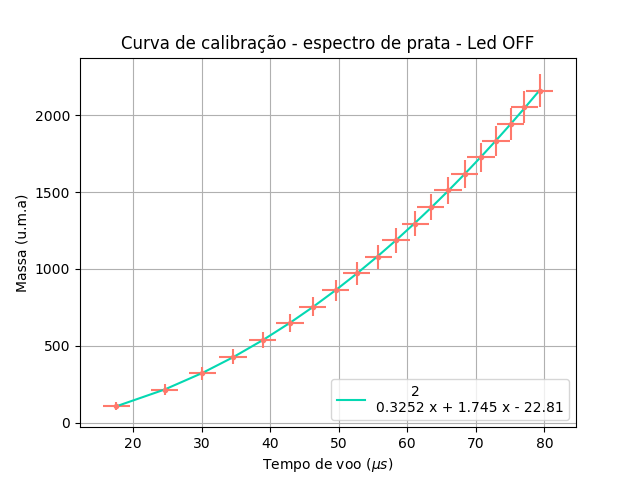
\includegraphics[width=0.7\textwidth]{exp_02/LEDOFF_curv+erro_calib.png}
  \caption{Curva de calibração para o LED ligado.}
  \label{fig:02_calib_ledOFF} 
\end{figure}

\begin{figure}
  \centering  
  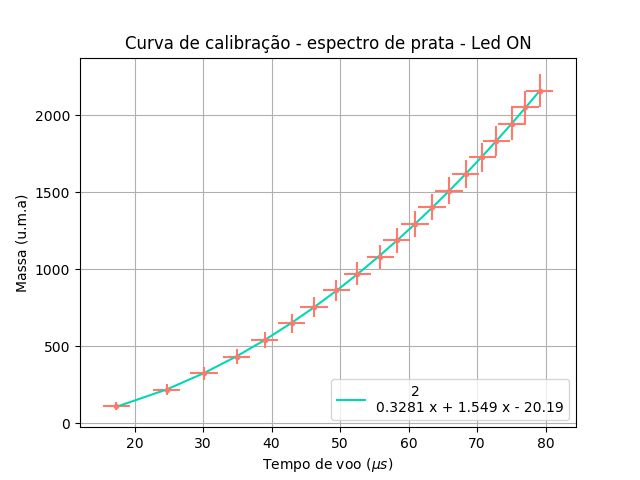
\includegraphics[width=0.7\textwidth]{exp_02/LEDON_curv+erro_calib.png}
  \caption{Curva de calibração para o LED ligado.}
  \label{fig:02_calib_ledON} 
\end{figure}

\begin{table}
\centering
\caption{Tempo de voo dos �tomos de Prata}
\label{tab:picos_encontados}
\begin{tabular}{|c|c|c|c|c|c|c|}
\hline
\begin{tabular}[c]{@{}c@{}}Prata\\ (N)\end{tabular} & \begin{tabular}[c]{@{}c@{}}Massa\\ te�rica\\ (u.m.a)\end{tabular} & \begin{tabular}[c]{@{}c@{}}LED OFF\\ Massa\\ calculada\\ $\pm \Delta m$\\ (u.m.a)\end{tabular} & \begin{tabular}[c]{@{}c@{}}LED ON\\ Massa\\ calculada\\ $\pm \Delta m$\\ (u.m.a)\end{tabular} & \begin{tabular}[c]{@{}c@{}}Tempo\\ te�rico\\ ($\mu s$)\end{tabular} & \begin{tabular}[c]{@{}c@{}}LED OFF\\ Tempo\\ calculado\\ $\pm \Delta t$\\ ($\mu s$)\end{tabular} & \begin{tabular}[c]{@{}c@{}}LED ON\\ Tempo\\ calculado\\ $\pm \Delta t$\\ ($\mu s$)\end{tabular} \\ \hline 
1&107.86&108$\pm$26&105$\pm$25&17.30&17$\pm$2&17$\pm$2\\ \hline 
2&215.72&216$\pm$35&217$\pm$35&24.47&24$\pm$2&24$\pm$2\\ \hline 
3&323.58&324$\pm$42&324$\pm$42&29.96&30$\pm$2&30$\pm$2\\ \hline 
4&431.44&426$\pm$48&433$\pm$48&34.60&34$\pm$2&34$\pm$2\\ \hline 
5&539.30&537$\pm$54&539$\pm$54&38.68&38$\pm$2&38$\pm$2\\ \hline 
6&647.16&651$\pm$59&650$\pm$59&42.38&42$\pm$2&42$\pm$2\\ \hline 
7&755.02&751$\pm$63&751$\pm$63&45.77&46$\pm$2&46$\pm$2\\ \hline 
8&862.88&862$\pm$67&859$\pm$68&48.93&49$\pm$2&49$\pm$2\\ \hline 
9&970.74&968$\pm$71&966$\pm$72&51.90&52$\pm$2&52$\pm$2\\ \hline 
10&1078.60&1087$\pm$76&1090$\pm$76&54.71&55$\pm$2&55$\pm$2\\ \hline 
11&1186.46&1186$\pm$79&1184$\pm$79&57.38&58$\pm$2&58$\pm$2\\ \hline 
12&1294.32&1300$\pm$83&1291$\pm$83&59.93&61$\pm$2&60$\pm$2\\ \hline 
13&1402.18&1395$\pm$85&1396$\pm$86&62.38&63$\pm$2&63$\pm$2\\ \hline 
14&1510.04&1507$\pm$89&1505$\pm$89&64.73&65$\pm$2&65$\pm$2\\ \hline 
15&1617.90&1616$\pm$92&1618$\pm$92&67.00&68$\pm$2&68$\pm$2\\ \hline 
16&1725.76&1728$\pm$95&1732$\pm$95&69.20&70$\pm$2&70$\pm$2\\ \hline 
17&1833.62&1833$\pm$98&1833$\pm$98&71.33&72$\pm$2&72$\pm$2\\ \hline 
18&1941.48&1941$\pm$101&1945$\pm$101&73.40&75$\pm$2&75$\pm$2\\ \hline 
19&2049.34&2043$\pm$103&2044$\pm$104&75.41&77$\pm$2&76$\pm$2\\ \hline 
20&2157.20&2161$\pm$106&2158$\pm$106&77.37&79$\pm$2&79$\pm$2\\ \hline 
\end{tabular} 
\end{table} 


Utilizando o processamento de dados foi obtido o espectro de partículas em função do tempo e em função da massa, como pode ser visto respectivamente nas Figuras \ref{fig:02_ledoff_dados_tratados}, \ref{fig:02_ledoff_massa}, \ref{fig:02_ledon_dados_tratados} e \ref{fig:02_ledon_massa}.

\begin{figure}
  \centering  
  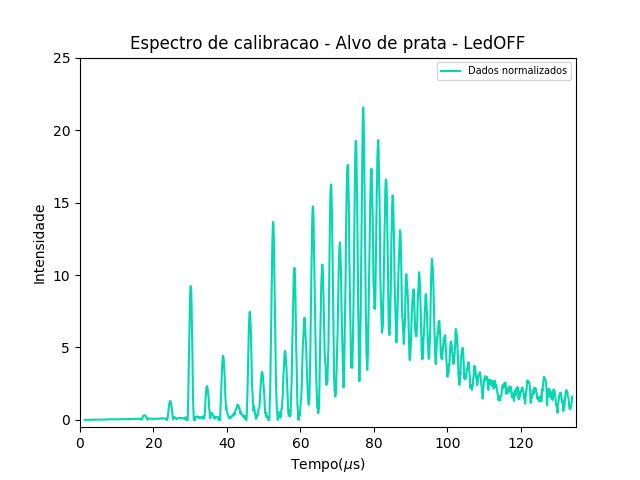
\includegraphics[width=0.7\textwidth]{exp_02/LEDOFF_normalizado_mcp.png}
  \caption{Espectro de calibração com tratamento de dados.}
  \label{fig:02_ledoff_dados_tratados} 
\end{figure}

\begin{figure}
  \centering  
  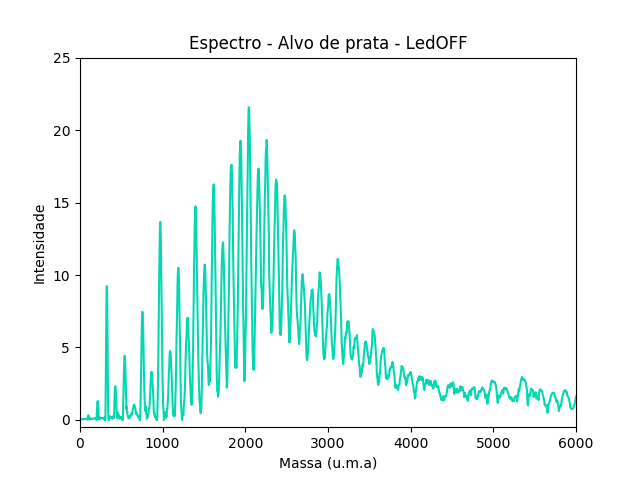
\includegraphics[width=0.7\textwidth]{exp_02/LEDOFF_espec_calib_ag_massa.png}
  \caption{Espectro de calibração com tratamento de dados.}
  \label{fig:02_ledoff_massa} 
\end{figure}



\begin{figure}
  \centering  
  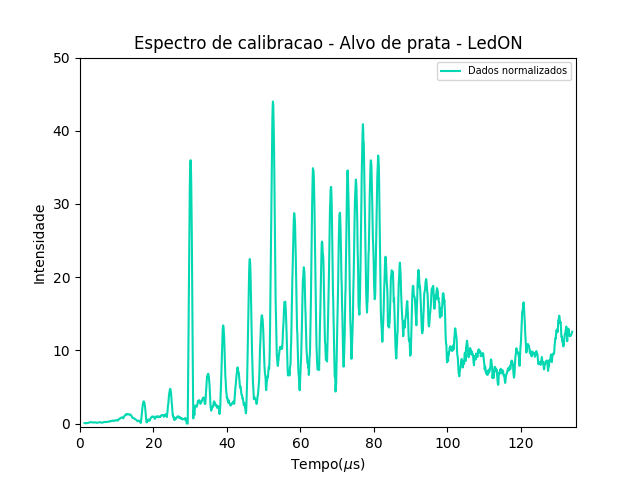
\includegraphics[width=0.7\textwidth]{exp_02/LEDON_normalizado_mcp.png}
  \caption{Espectro de calibração com tratamento de dados.}
  \label{fig:02_ledon_dados_tratados} 
\end{figure}

\begin{figure}
  \centering  
  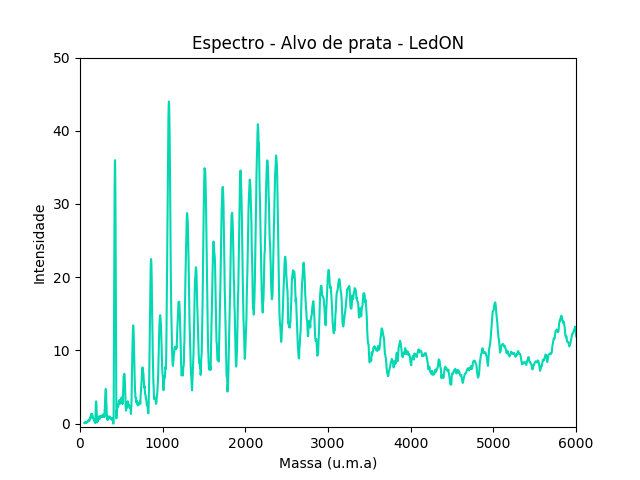
\includegraphics[width=0.7\textwidth]{exp_02/LEDON_espec_calib_ag_massa.png}
  \caption{Espectro de calibração com tratamento de dados.}
  \label{fig:02_ledon_massa} 
\end{figure}

\section{Experimento III}
A tabela e os dados utilizados para a calibração de ambos os estados do LED, pode ser vista na Tabela \ref{tab:picos_encontados_03}, assim como as curvas de calibração dos espectros que correspondem as Figuras \ref{fig:03_calib_ledOFF} e \ref{fig:03_calib_ledON}.

\begin{figure}
  \centering  
  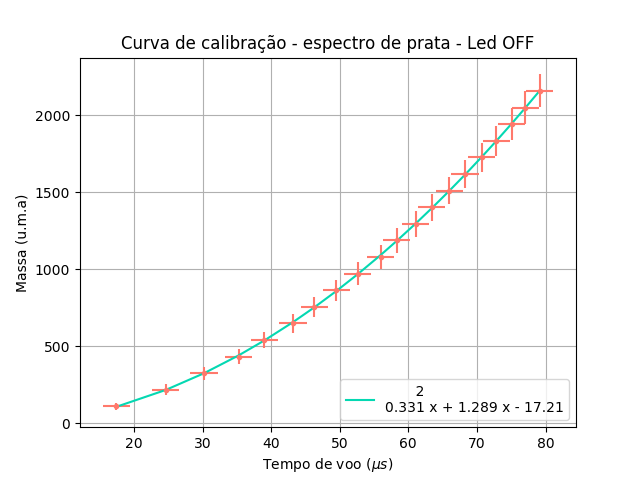
\includegraphics[width=0.7\textwidth]{exp_03/LEDOFF_curv+erro_calib.png}
  \caption{Curva de calibração para o LED ligado.}
  \label{fig:03_calib_ledOFF} 
\end{figure}

\begin{figure}
  \centering  
  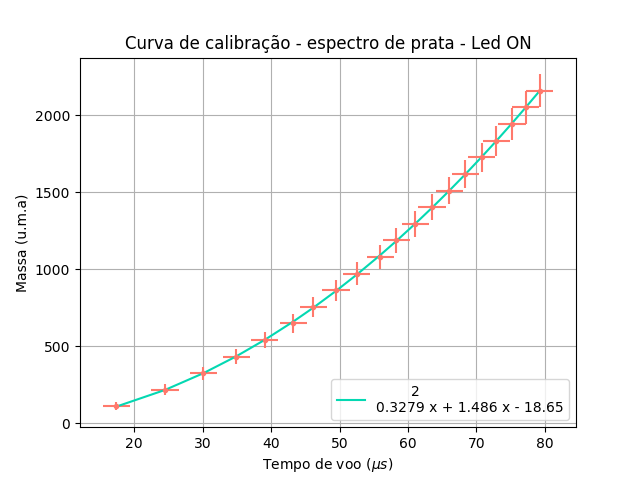
\includegraphics[width=0.7\textwidth]{exp_03/LEDON_curv+erro_calib.png}
  \caption{Curva de calibração para o LED ligado.}
  \label{fig:03_calib_ledON} 
\end{figure}

\begin{table}
\centering
\caption{Tempo de voo dos átomos de Prata}
\label{tab:picos_encontados_03}
\begin{tabular}{|c|c|c|c|c|c|c|}
\hline
\begin{tabular}[c]{@{}c@{}}Prata\\ (N)\end{tabular} & \begin{tabular}[c]{@{}c@{}}Massa\\ teórica\\ (u.m.a)\end{tabular} & \begin{tabular}[c]{@{}c@{}}LED OFF\\ Massa\\ calculada\\ $\pm \Delta m$\\ (u.m.a)\end{tabular} & \begin{tabular}[c]{@{}c@{}}LED ON\\ Massa\\ calculada\\ $\pm \Delta m$\\ (u.m.a)\end{tabular} & \begin{tabular}[c]{@{}c@{}}Tempo\\ teórico\\ ($\mu s$)\end{tabular} & \begin{tabular}[c]{@{}c@{}}LED OFF\\ Tempo\\ calculado\\ $\pm \Delta t$\\ ($\mu s$)\end{tabular} & \begin{tabular}[c]{@{}c@{}}LED ON\\ Tempo\\ calculado\\ $\pm \Delta t$\\ ($\mu s$)\end{tabular} \\ \hline 
1&107.86&105$\pm$25&106$\pm$25&17.30&17$\pm$2&17$\pm$2\\ \hline 
2&215.72&214$\pm$35&214$\pm$35&24.47&24$\pm$2&24$\pm$2\\ \hline 
3&323.58&323$\pm$42&323$\pm$42&29.96&30$\pm$2&30$\pm$2\\ \hline 
4&431.44&439$\pm$49&433$\pm$48&34.60&35$\pm$2&34$\pm$2\\ \hline 
5&539.30&536$\pm$54&540$\pm$54&38.68&38$\pm$2&39$\pm$2\\ \hline 
6&647.16&655$\pm$59&658$\pm$59&42.38&43$\pm$2&43$\pm$2\\ \hline 
7&755.02&751$\pm$63&749$\pm$63&45.77&46$\pm$2&46$\pm$2\\ \hline 
8&862.88&856$\pm$68&857$\pm$67&48.93&49$\pm$2&49$\pm$2\\ \hline 
9&970.74&966$\pm$72&963$\pm$71&51.90&52$\pm$2&52$\pm$2\\ \hline 
10&1078.60&1091$\pm$76&1091$\pm$76&54.71&55$\pm$2&55$\pm$2\\ \hline 
11&1186.46&1182$\pm$79&1181$\pm$79&57.38&58$\pm$2&58$\pm$2\\ \hline 
12&1294.32&1296$\pm$83&1295$\pm$83&59.93&61$\pm$2&61$\pm$2\\ \hline 
13&1402.18&1395$\pm$86&1396$\pm$86&62.38&63$\pm$2&63$\pm$2\\ \hline 
14&1510.04&1507$\pm$89&1509$\pm$89&64.73&65$\pm$2&66$\pm$2\\ \hline 
15&1617.90&1614$\pm$92&1615$\pm$92&67.00&68$\pm$2&68$\pm$2\\ \hline 
16&1725.76&1727$\pm$96&1728$\pm$95&69.20&70$\pm$2&70$\pm$2\\ \hline 
17&1833.62&1832$\pm$99&1833$\pm$98&71.33&72$\pm$2&72$\pm$2\\ \hline 
18&1941.48&1945$\pm$101&1945$\pm$101&73.40&75$\pm$2&75$\pm$2\\ \hline 
19&2049.34&2048$\pm$104&2048$\pm$104&75.41&77$\pm$2&77$\pm$2\\ \hline 
20&2157.20&2159$\pm$107&2157$\pm$106&77.37&79$\pm$2&79$\pm$2\\ \hline 
\end{tabular} 
\end{table} 


Utilizando o processamento de dados foi obtido o espectro de partículas em função do tempo e em função da massa, como pode ser visto respectivamente nas Figuras \ref{fig:03_ledoff_dados_tratados}, \ref{fig:03_ledoff_massa}, \ref{fig:03_ledon_dados_tratados} e \ref{fig:03_ledon_massa}.

\begin{figure}
  \centering  
  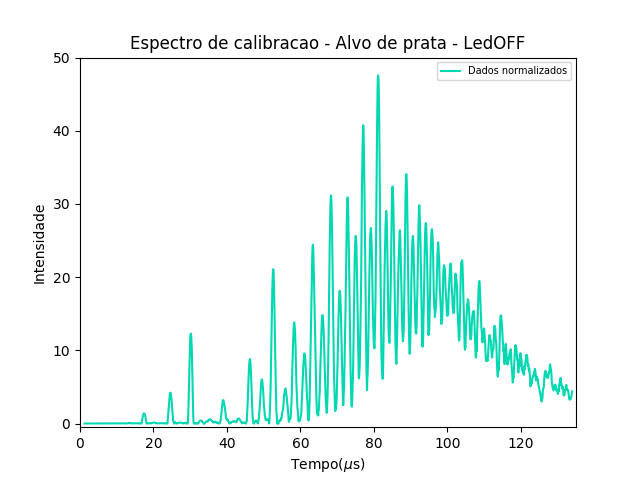
\includegraphics[width=0.7\textwidth]{exp_03/LEDOFF_normalizado_mcp.png}
  \caption{Espectro de calibração com tratamento de dados.}
  \label{fig:03_ledoff_dados_tratados} 
\end{figure}

\begin{figure}
  \centering  
  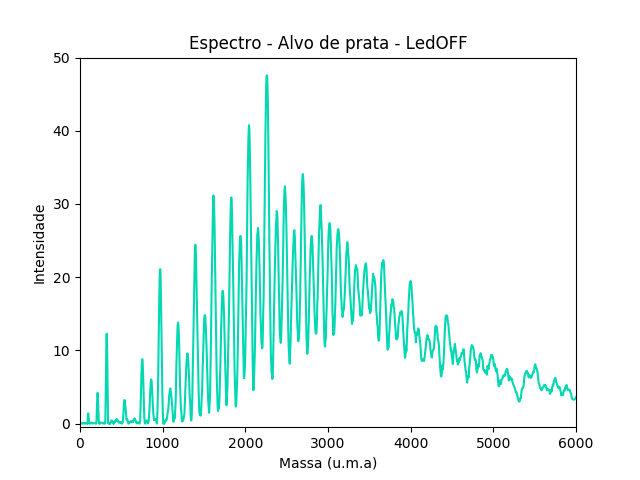
\includegraphics[width=0.7\textwidth]{exp_03/LEDOFF_espec_calib_ag_massa.png}
  \caption{Espectro de calibração com tratamento de dados.}
  \label{fig:03_ledoff_massa} 
\end{figure}



\begin{figure}
  \centering  
  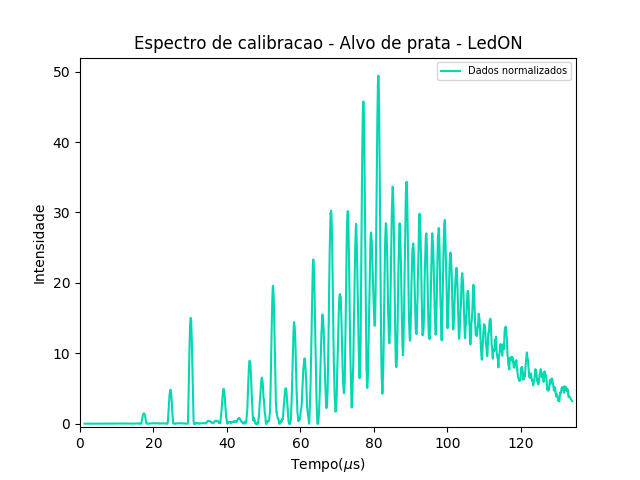
\includegraphics[width=0.7\textwidth]{exp_03/LEDON_normalizado_mcp.png}
  \caption{Espectro de calibração com tratamento de dados.}
  \label{fig:03_ledon_dados_tratados} 
\end{figure}

\begin{figure}
  \centering  
  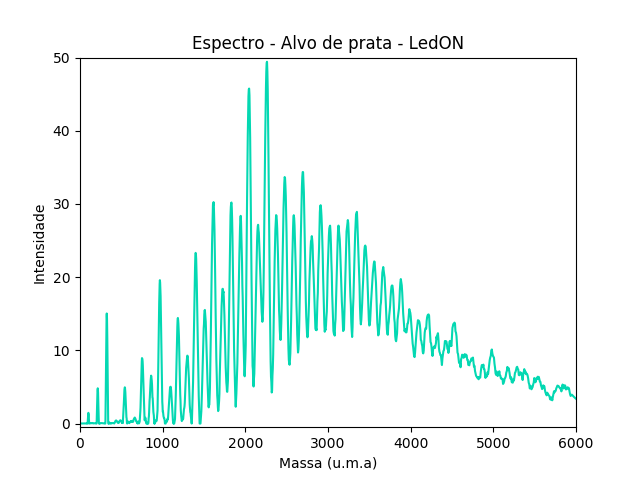
\includegraphics[width=0.7\textwidth]{exp_03/LEDON_espec_calib_ag_massa.png}
  \caption{Espectro de calibração com tratamento de dados.}
  \label{fig:03_ledon_massa} 
\end{figure}

\section{Experimento IV}
A tabela e os dados utilizados para a calibração de ambos os estados do LED, pode ser vista na Tabela \ref{tab:picos_encontados_04}, assim como as curvas de calibração dos espectros que correspondem as Figuras \ref{fig:04_calib_ledOFF} e \ref{fig:04_calib_ledON}.

\begin{figure}
  \centering  
  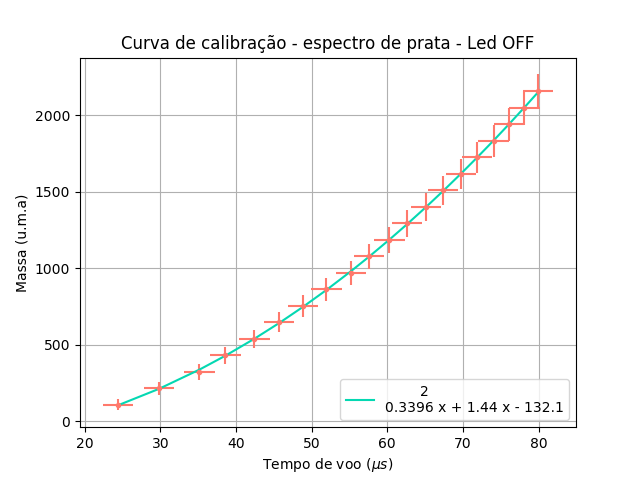
\includegraphics[width=0.7\textwidth]{exp_04/LEDOFF_curv+erro_calib.png}
  \caption{Curva de calibração para o LED ligado.}
  \label{fig:04_calib_ledOFF} 
\end{figure}

\begin{figure}
  \centering  
  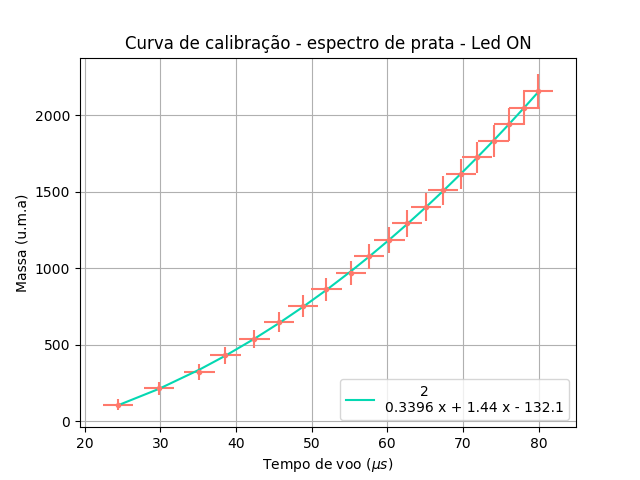
\includegraphics[width=0.7\textwidth]{exp_04/LEDON_curv+erro_calib.png}
  \caption{Curva de calibração para o LED ligado.}
  \label{fig:04_calib_ledON} 
\end{figure}

\begin{table}
\centering
\caption{Tempo de voo dos átomos de Prata}
\label{tab:picos_encontados_04}
\begin{tabular}{|c|c|c|c|c|c|c|}
\hline
\begin{tabular}[c]{@{}c@{}}Prata\\ (N)\end{tabular} & \begin{tabular}[c]{@{}c@{}}Massa\\ teórica\\ (u.m.a)\end{tabular} & \begin{tabular}[c]{@{}c@{}}LED OFF\\ Massa\\ calculada\\ $\pm \Delta m$\\ (u.m.a)\end{tabular} & \begin{tabular}[c]{@{}c@{}}LED ON\\ Massa\\ calculada\\ $\pm \Delta m$\\ (u.m.a)\end{tabular} & \begin{tabular}[c]{@{}c@{}}Tempo\\ teórico\\ ($\mu s$)\end{tabular} & \begin{tabular}[c]{@{}c@{}}LED OFF\\ Tempo\\ calculado\\ $\pm \Delta t$\\ ($\mu s$)\end{tabular} & \begin{tabular}[c]{@{}c@{}}LED ON\\ Tempo\\ calculado\\ $\pm \Delta t$\\ ($\mu s$)\end{tabular} \\ \hline 
1&107.86&104$\pm$35&104$\pm$35&17.30&24$\pm$2&24$\pm$2\\ \hline 
2&215.72&212$\pm$43&212$\pm$43&24.47&29$\pm$2&29$\pm$2\\ \hline 
3&323.58&338$\pm$50&338$\pm$50&29.96&35$\pm$2&35$\pm$2\\ \hline 
4&431.44&429$\pm$55&429$\pm$55&34.60&38$\pm$2&38$\pm$2\\ \hline 
5&539.30&540$\pm$60&540$\pm$60&38.68&42$\pm$2&42$\pm$2\\ \hline 
6&647.16&643$\pm$64&643$\pm$64&42.38&45$\pm$2&45$\pm$2\\ \hline 
7&755.02&748$\pm$69&748$\pm$69&45.77&48$\pm$2&48$\pm$2\\ \hline 
8&862.88&859$\pm$73&859$\pm$73&48.93&51$\pm$2&51$\pm$2\\ \hline 
9&970.74&980$\pm$77&980$\pm$77&51.90&55$\pm$2&55$\pm$2\\ \hline 
10&1078.60&1075$\pm$81&1075$\pm$81&54.71&57$\pm$2&57$\pm$2\\ \hline 
11&1186.46&1188$\pm$84&1188$\pm$84&57.38&60$\pm$2&60$\pm$2\\ \hline 
12&1294.32&1288$\pm$87&1288$\pm$87&59.93&62$\pm$2&62$\pm$2\\ \hline 
13&1402.18&1403$\pm$91&1403$\pm$91&62.38&65$\pm$2&65$\pm$2\\ \hline 
14&1510.04&1507$\pm$94&1507$\pm$94&64.73&67$\pm$2&67$\pm$2\\ \hline 
15&1617.90&1618$\pm$97&1618$\pm$97&67.00&69$\pm$2&69$\pm$2\\ \hline 
16&1725.76&1725$\pm$100&1725$\pm$100&69.20&71$\pm$2&71$\pm$2\\ \hline 
17&1833.62&1836$\pm$103&1836$\pm$103&71.33&74$\pm$2&74$\pm$2\\ \hline 
18&1941.48&1940$\pm$106&1940$\pm$106&73.40&76$\pm$2&76$\pm$2\\ \hline 
19&2049.34&2052$\pm$108&2052$\pm$108&75.41&78$\pm$2&78$\pm$2\\ \hline 
20&2157.20&2154$\pm$111&2154$\pm$111&77.37&79$\pm$2&79$\pm$2\\ \hline 
\end{tabular} 
\end{table} 


Utilizando o processamento de dados foi obtido o espectro de partículas em função do tempo e em função da massa, como pode ser visto respectivamente nas Figuras \ref{fig:04_ledoff_dados_tratados}, \ref{fig:04_ledoff_massa}, \ref{fig:04_ledon_dados_tratados} e \ref{fig:04_ledon_massa}.

\begin{figure}
  \centering  
  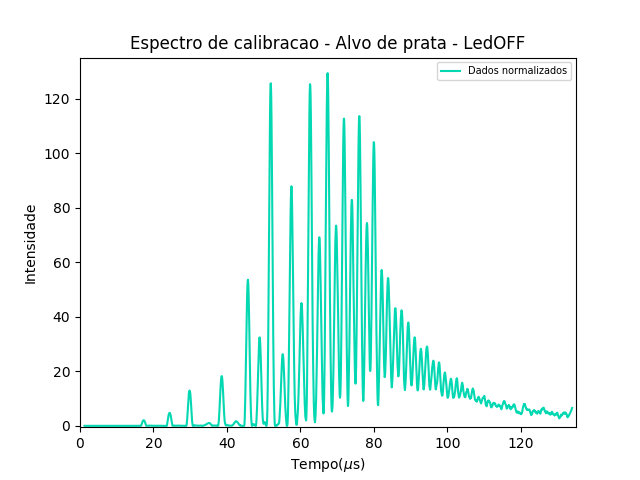
\includegraphics[width=0.7\textwidth]{exp_04/LEDOFF_normalizado_mcp.png}
  \caption{Espectro de calibração com tratamento de dados.}
  \label{fig:04_ledoff_dados_tratados} 
\end{figure}

\begin{figure}
  \centering  
  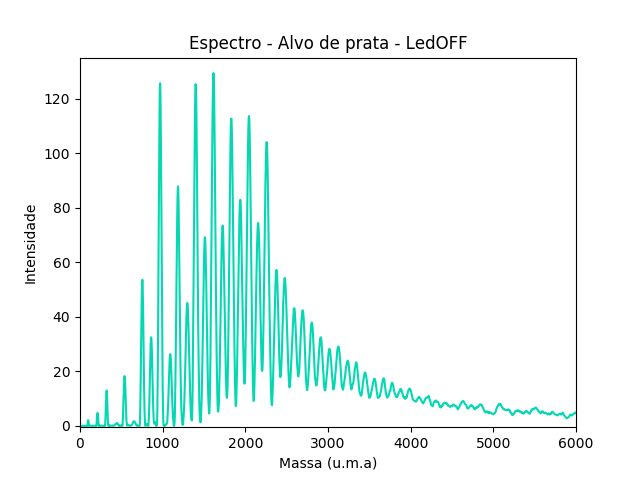
\includegraphics[width=0.7\textwidth]{exp_04/LEDOFF_espec_calib_ag_massa.png}
  \caption{Espectro de calibração com tratamento de dados.}
  \label{fig:04_ledoff_massa} 
\end{figure}



\begin{figure}
  \centering  
  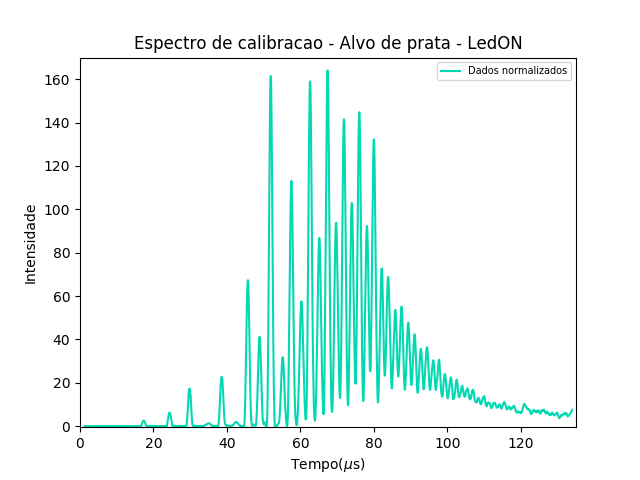
\includegraphics[width=0.7\textwidth]{exp_04/LEDON_normalizado_mcp.png}
  \caption{Espectro de calibração com tratamento de dados.}
  \label{fig:04_ledon_dados_tratados} 
\end{figure}

\begin{figure}
  \centering  
  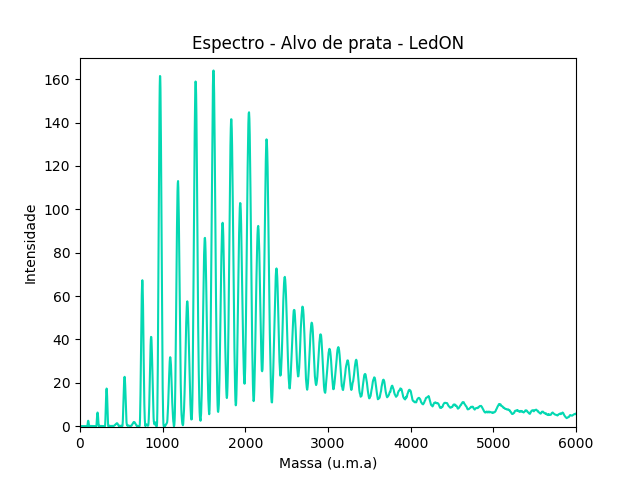
\includegraphics[width=0.7\textwidth]{exp_04/LEDON_espec_calib_ag_massa.png}
  \caption{Espectro de calibração com tratamento de dados.}
  \label{fig:04_ledon_massa} 
\end{figure}

